% 4º LEIC Estudante Edmilson Gil De Carvalho Fernandes
% edmilsongilfernandes@student.unicv.edu.cv 
% 4º ano EIC
\documentclass[a4paper,12pt]{report}
\usepackage[utf8]{inputenc}
\usepackage[hidelinks]{hyperref}
\DeclareUnicodeCharacter{202F}{~}
\DeclareUnicodeCharacter{2194}{\ensuremath{\leftrightarrow}}
\DeclareUnicodeCharacter{2248}{\ensuremath{\approx}}
\usepackage{graphicx}
\usepackage{background}
\usepackage[toc, acronym]{glossaries}
\usepackage{amsmath}
\usepackage{array}
\usepackage{pgfplots}
\pgfplotsset{compat=1.18}
\usetikzlibrary{positioning, arrows.meta, calc, shapes.geometric}
\usepackage[lmargin=2cm,tmargin=2cm,rmargin=2cm,bmargin=2cm]{geometry}
\usepackage{xcolor}
\usepackage{multirow}
\usepackage{multicol}
\usepackage{indentfirst}
\usepackage{booktabs}
\usepackage{float}
\usepackage[onehalfspacing]{setspace}
\usepackage[portuges]{babel}
\usepackage{datetime}
\usepackage[T1]{fontenc}
\usepackage{ragged2e}
\usepackage{url}

\selectlanguage{portuges}

\newdateformat{monthyeardate}{ \monthname[\THEMONTH], \THEYEAR}

 %   Imagen na fundo
\backgroundsetup{scale=1, angle=0, opacity=1, contents={
\includegraphics[scale=1]{figuras/tfc background.jpg }}}

% Glossário
\newglossaryentry{ovs}{
    name={OVS},
    description={Open vSwitch}
}

\makeglossaries

\begin{document}

\pagenumbering{gobble}

% Capa
\BgThispage
\begin{center}
% Página com imagem de fundo
    
\includegraphics[width=10cm, height=5cm]{figuras/unicv_fct.png} % Verifique se o caminho está correto
    \begin{minipage}{.9\textwidth}
        \centering
        \vspace{-0.5cm}
        \textbf{UNIVERSIDADE DE CABO VERDE}\\
        {FACULDADE DE CIÊNCIAS E TECNOLOGIA}\\
        {LICENCIATURA EM ENGENHARIA ELETROTÉCNICA}
    \end{minipage}
    
    % Tema
    \vspace{3cm}
    \huge{\textbf{Blockchain em uma nova abordagem em sistema de votações eletrónicas}}

    \vspace{4cm}
    \large
    \begin{tabular}{c}
        \textsl{\LARGE{\color{white} Edmilson Gil De Carvalho Fernandes }}\\
        \textrm{\color{white}{Orientador}: Prof. Dr. Celestino Lopes de Barros}
    \end{tabular}
    
    \vspace{6cm}
    \color{white}Campus Palmarejo Grande, Praia, \monthyeardate \today
    % Página específica com fundo
\backgroundsetup{
  contents={
\includegraphics[scale=1]{figuras/tfc background.jpg}}
}

\end{center}

 \newpage
% Página de título
\NoBgThispage
\begin{center}

    \begin{figure}
        \centering
        
\includegraphics[width=0.5\linewidth]{figuras/unicv_fct.png} % Verifique se o caminho está correto
        \label{fig:enter-label}
    \end{figure}
    \begin{minipage}{.9\textwidth}
        \centering
        \vspace{0.5cm}
        \textbf{UNIVERSIDADE DE CABO VERDE}\\
        \textbf{FACULDADE DE CIÊNCIAS E TECNOLOGIA}\\
        \textbf{LICENCIATURA EM ENGENHARIA INFORMÁTICA E DE COMPUTADORES}
    \end{minipage}
    
    % Tema
    \vspace{2.5cm}
    \LARGE{\textbf{Blockchain em uma nova abordagem em sistema de votações eletrónicas}}
\end{center}

\vspace{1.5cm}
\begin{flushright}
    Projeto sobre uma nova\\ 
    abordagem em sistema\\
    de votações eletrónicas \\
    desenvolvido durante o Trabalho\\
    Final do Curso, apresentado à\\
    Universidade de Cabo Verde para\\ 
    obtenção do grau de Licenciatura\\ 
    em Engenharia Informática e de\\
    Computadores.
\end{flushright}
\NoBgThispage
\begin{center}
    \vspace{1.5cm}
    {\large
        \textbf{Edmilson Gil De Carvalho Fernandes} \\
        \begin{tabular}{rl}
            {Orientador}: & \textbf{Prof. Dr. Celestino Lopes de Barros}
        \end{tabular}
    }
\end{center}

\newpage

% Página de aprovação
\begin{center}
    Praia, \today
    
    \vspace{1cm}
    Trabalho Fim de Curso (TFC) apresentado à Universidade de Cabo Verde (UNICV) sob título Blockchain em uma nova abordagem em sistema de votações eletrónicas
    
    \vspace{1.5cm}
    \textbf{Elaborado Por}: Edmilson Gil De Carvalho Fernandes
    
    \vspace{1.5cm}
    É aprovado pelos membros do júri, como requisito parcial à obtenção do grau de Licenciatura em Engenharia Informática e de Computadores.
    
    \vspace{1.5cm}
    \textbf{Presidente}\\
    \vspace{1.5cm}
    ----------------------------------------------------------------------\\
    \vspace{1.5cm}
    \textbf{Arguente:}\\
    \vspace{1.5cm}
    ----------------------------------------------------------------------\\
    \vspace{1.5cm}
    \textbf{Orientador:}\\
    \vspace{1.5cm}
    ----------------------------------------------------------------------\\
    \vspace{1cm}
    \textbf{Data}\\
    \vspace{1cm}
    Praia, \textunderscore\textunderscore\textunderscore\textunderscore\textunderscore/
            \textunderscore\textunderscore\textunderscore\textunderscore\textunderscore/
            \textunderscore\textunderscore\textunderscore\textunderscore\textunderscore
\end{center}

\newpage

\pagenumbering{roman}

% Incluir agradecimentos
%Creditos para o Prof.Hernâni D. Chantre 
%hernani.chantre@docente.unicv.edu.cv 
%4º LEIC Estudante Cláudio Micheal Moreira
%claudiom.moreira@student.unicv.edu.cv 
%4ºano TMC Elias Souto
%jose.souto@student.unicv.edu.cv 

%\textbf{Agradecimentos}


\begin{center} 
    \large{Agradecimentos} 
\end{center}
   
\justifying{

Agradeço primeiramente a Deus, por me dar força e sabedoria para concluir este curso. À minha mãe, \textbf{Benedita}, que sempre me apoiou e acreditou em mim, mesmo nos momentos mais difíceis.

Agradeço aos meus irmãos e irmã, que sempre estiveram ao meu lado, em especial ao meu irmão \textbf{Cesaltino}, cujo apoio foi inestimável durante esta jornada.

Aos meus primos e primas, agradeço por todo o encorajamento e apoio, em especial à minha prima \textbf{Ederlina}, ao meu primo \textbf{Ederlino} e à minha prima \textbf{Ludneida}. Vocês foram verdadeiros pilares de apoio para mim.

À minha tia \textbf{Silvina}, agradeço por todas as palavras de incentivo e pela fé que sempre teve em mim.

A todos os meus familiares e amigos que contribuíram, de uma forma ou de outra, para a realização deste trabalho, o meu mais sincero obrigado. Este trabalho é também um reflexo do amor e do apoio que vocês me deram.

Por fim, agradeço a todos os professores e colegas que fizeram parte desta jornada. Sem vocês, este trabalho não seria possível.

}


% Introduzir Resumo
\begin{center} \large{Resumo} \end{center}
    \justifying{
    
    A sociedade evoluiu de acordo com o crescimento da tecnologia, de modo que comportamentos sociais complexos foram influenciados por ela. Nesse contexto, o sistema de vota{\c{c}}{\~a}o eletr{\'o}nica surge como uma evolu{\c{c}}{\~a}o natural. No entanto, o desenvolvimento de tais sistemas n{\~a}o deve focar apenas na contagem de votos, mas deve respeitar rigorosamente os fundamentos do sufr{\'a}gio, sendo este {\'u}nico por pessoa, privado e secreto.
}
    
    \vspace{0.8cm}
    {\sloppy \textbf{Palavras-Chave:} \emph{Blockchain; Vota{\c{c}}{\~a}o; Eletr{\'o}nica; Smart Contracts; Auditabilidade; Web3}.\par}
    
    \vspace{2.5cm}

\newpage

% Introduzir Abstract
\begin{center} \large{Abstract} \end{center}

This work explores a novel approach to electronic voting systems by integrating blockchain technology to enhance security, transparency, and voter trust. Traditional voting mechanisms face critical challenges such as human error, fraud, high costs, and limited accessibility. By leveraging the decentralized and immutable nature of blockchain, the proposed system ensures each vote is unique, verifiable, and securely recorded on-chain. Through a detailed literature review and system design proposal, the study outlines the architecture of a smart contract-powered voting platform, including voter authentication, election lifecycle management, and real-time result tracking. The implementation also considers user interface design, usability, and legal/ethical implications. This project contributes not only by proposing a secure, transparent, and auditable voting method but also by laying a foundation for future research in democratic digital transformation using decentralized technologies.

\vspace{0.8cm}
\textbf{Key Words:} Blockchain, Electronic Voting, Smart Contracts, Auditability, Web3.

\newpage

\renewcommand{\listtablename}{Lista de Figuras}
\addcontentsline{toc}{chapter}{\listtablename}
\listoffigures

\newpage

\renewcommand{\listtablename}{Lista de Tabelas}
\addcontentsline{toc}{chapter}{\listtablename}
\listoftables

\newpage

% Lista de Abreviaturas e Siglas
\printglossary[title=Lista de Abreviaturas e Siglas, type=\acronymtype]

\newpage

\tableofcontents

\newpage
% Página específica com fundo
%\backgroundsetup{
 % contents={
\includegraphics[scale=1]{figuras/tfc background.jpg}}}

% Incluir capítulos reorganizados
% Capítulo 1 – Introdução (copiado de cap_Intro.tex)
\chapter{Introdução}\label{cap1}
\justifying
A democracia é definida como o direito das pessoas de escolherem os seus líderes. A votação é um processo crítico que permite às pessoas elegerem o seu líder governamental. O sistema eleitoral deve ser democrático, independente e imparcial. Como resultado, deve ser um procedimento transparente e seguro que permita a todos partilhar livremente o seu ponto de vista.\cite{alvi_dvtchain_2022}

Dito isso, e com a evolução tecnológica tem impulsionado mudanças significativas em diversos setores da sociedade, e o sistema de votações eletrónicas não fica de fora.

Existem diferentes meios de votação pelo mundo, sendo o mais comum a votação em papel. Este sistema utiliza cédulas físicas que o eleitor marca em centros designados, sob observação de auditores, mas mantendo o sigilo do voto. As cédulas são depositadas em urnas e contadas manualmente, um processo demorado que exige recursos humanos substanciais e acarreta riscos de segurança, além de dificuldades de armazenamento e acessibilidade para idosos ou pessoas com mobilidade reduzida.\cite{hajian_berenjestanaki_blockchain-based_2024}

Considerando as desvantagens acima mencionadas, os métodos de votação evoluíram muito com o avanço das Tecnologias de Informação e Comunicação (TIC).

Nas últimas décadas, houve uma crescente busca por métodos mais eficientes, seguros e transparentes para acompanhar os processos eleitorais. Nesse contexto, a tecnologia Blockchain surge como uma solução promissora para melhorar a integridade e confiabilidade das votações eletrónicas.

\newpage

\section{Enquadramento e Justificação}

A tecnologia Blockchain tem sido amplamente reconhecida pela sua capacidade de fornecer transparência, segurança e imutabilidade. Estas características tornam a Blockchain uma candidata promissora para resolver muitos dos desafios enfrentados pelos sistemas de votação electrónica, como a manipulação de votos, a falta de transparência e a vulnerabilidade a ataques cibernéticos.

O sistema de votação electrónica actual enfrenta vários desafios, incluindo a falta de confiança do público, a possibilidade de fraude e a falta de transparência no processo de votação. A tecnologia Blockchain, com a sua natureza descentralizada e imutável, oferece uma solução potencial para estes problemas.

Este projecto propõe uma nova abordagem para o sistema de votação electrónica utilizando a tecnologia Blockchain. O objectivo é desenvolver um sistema de votação que seja seguro, transparente e imune a fraudes. Acreditamos que a implementação da tecnologia Blockchain no sistema de votação electrónica pode aumentar a confiança do público no processo de votação, garantindo que cada voto seja contado correctamente e que o processo de votação seja transparente e verificável.

Além disso, este trabalho contribuirá para a literatura existente sobre o uso da tecnologia Blockchain em sistemas de votação electrónica, fornecendo uma análise abrangente dos desafios enfrentados e das soluções propostas. Esperamos que este trabalho sirva como um recurso valioso para investigadores e profissionais interessados em explorar o potencial da tecnologia Blockchain para melhorar os sistemas de votação electrónica.

% Problema de Investigação
\section{Problema de Investigação}

A digitalização dos processos eleitorais tem impulsionado a adoção de sistemas de votação eletrónica centralizados. Embora esses sistemas aumentem a eficiência logística, apresentam três falhas críticas:

\begin{enumerate}
    \item \textbf{Opacidade algorítmica}: os algoritmos que contabilizam e validam os votos são proprietários, impedindo auditorias independentes.
    \item \textbf{Vulnerabilidade a ataques internos}: a centralização de dados e chaves criptográficas cria um ponto único de falha, facilitando a manipulação de resultados.
    \item \textbf{Ausência de anonimato verificável}: a maioria das soluções não garante que o voto seja anônimo ao mesmo tempo em que permite rastreabilidade para fins de auditoria.
\end{enumerate}

Consequentemente, o problema central desta investigação é:

\begin{quote}
\textit{Como integrar Smart Contracts e arquiteturas Web3 de forma a garantir, simultaneamente, a integridade imutável do voto, o anonimato do eleitor e a transparência total do apuramento, sem depender de uma autoridade central de confiança?}
\end{quote}

Esta questão orienta a busca por um artefacto (VotoChain) que supra as limitações dos sistemas atuais, oferecendo:
\begin{itemize}
    \item \textbf{Descentralização total} dos registros de voto mediante blockchain pública (Ethereum Sepolia);
    \item \textbf{Anonimato criptográfico} suportado por técnicas de zero-knowledge proof (ZKP) ou mix-nets;
    \item \textbf{Auditabilidade pública} por meio de contratos inteligentes verificáveis e logs imutáveis.
\end{itemize}

% Objetivos e Contribuições
\section{Objetivos e Contribuições}

\subsection{Objetivo Geral}
Desenvolver e avaliar um protótipo de sistema de votação eletrónica (VotoChain) baseado na tecnologia blockchain (EVM) que assegure a viabilidade técnica de:
\begin{enumerate}
    \item Integridade e imutabilidade dos votos;
    \item Anonimato verificável do eleitor;
    \item Transparência e auditabilidade pública sem a necessidade de uma autoridade central.
\end{enumerate}

\subsection{Objetivos Específicos}
\begin{enumerate}
    \item Revisão sistemática da literatura para mapear vulnerabilidades e mecanismos de segurança de sistemas de votação eletrónica existentes, identificando lacunas nas áreas de anonimato, auditabilidade e descentralização.
    \item Projeto e implementação de smart contracts robustos em Solidity que gerenciem o ciclo de vida da eleição (registro, votação, apuração) e garantam a unicidade do voto por meio de identidades digitais.
    \item Integração de um mecanismo de anonimato criptográfico (ZKP ou mix‑nets) para dissociar a identidade do eleitor do voto, mantendo a verificabilidade.
    \item Desenvolvimento de uma interface acessível (React + Ethers.js) que siga as diretrizes WCAG 2.1, permitindo a participação inclusiva de usuários com diferentes necessidades.
    \item Avaliação quantitativa dos custos de \textit{gas}, latência de transação e taxa de falhas em ambiente de teste (Sepolia) e comparação com soluções comerciais (Voatz, Helios, POLYAS).
    \item Validação qualitativa por meio de testes de usabilidade com usuários reais, coletando feedback sobre confiança, percepção de segurança e experiência de voto.
\end{enumerate}

\subsection{Contribuições}
\begin{enumerate}
    \item \textbf{Metodológica}: aplicação do framework \textit{Design Science Research} (DSR) para o desenvolvimento rigoroso de artefatos tecnológicos em contextos eleitorais.
    \item \textbf{Técnica}: implementação de um modelo híbrido de autenticação que associa identidades institucionais a endereços Ethereum, aliado a um mecanismo de anonimato criptográfico.
    \item \textbf{Social}: demonstração de design universal e acessibilidade digital em um sistema de votação Web3, reduzindo barreiras de participação.
    \item \textbf{Estado da Arte}: análise comparativa crítica entre VotoChain e soluções existentes (Voatz, Helios, POLYAS), evidenciando requisitos ainda não atendidos (ex.: escalabilidade de ZKP, auditoria em tempo real).
\end{enumerate}

% Metodologia de investigação
\section{Metodologia de Investigação}

Para que um conhecimento possa ser considerado científico, torna‑se necessário identificar as operações mentais e técnicas que possibilitam a sua verificação (GIL, 2008).\cite{prodanov2013metodologia} O principal objetivo da investigação científica é, justamente, o de saber se essa sugestão apresentada, isto é, a hipótese, enquanto enunciado objetivo e independente do pesquisador, será corroborada ou falseada. E embora corroborada, ela sempre manterá o caráter hipotético. Para \textit{Kerlinger}, “as hipóteses são uma ferramenta poderosa para o avanço do conhecimento porque, embora formuladas pelo homem, podem ser testadas e mostradas como provavelmente corretas ou incorretas, à parte dos valores e crenças do homem” (1985, p. 40).

Apresenta‑se aqui um projeto que tem a função de \textbf{"Utilização de Blockchain em uma nova abordagem em sistema de votações eletrónicas"}.

% Estrutura de trabalho
\section{Estrutura de Trabalho}
\begin{description}
    \item[Capítulo I: Introdução] Apresenta o contexto, motivação, problema de investigação, objetivos e as contribuições do trabalho.
    \item[Capítulo II: Estado da Arte] Fornece uma revisão crítica da literatura sobre plataformas de votação blockchain, técnicas de anonimato e análise de desempenho.
    \item[Capítulo III: Metodologia de Investigação] Detalha a aplicação do framework \textit{Design Science Research} (DSR) e as fases de desenvolvimento do artefacto.
    \item[Capítulo IV: Proposta de Arquitetura e Design] Descreve a arquitetura técnica do VotoChain, os smart contracts, o módulo de anonimato e o design de interface (WCAG 2.1).
    \item[Capítulo V: Resultados e Validação] Apresenta os dados quantitativos (gas, latência) e qualitativos (SUS, acessibilidade) obtidos nos experimentos.
    \item[Capítulo VI: Discussão Crítica] Analisa os resultados frente às ameaças à validade, limitações técnicas e comparações com o estado da arte.
    \item[Capítulo VII: Conclusão e Trabalhos Futuros] Sintetiza as conclusões, contribuições e propõe um roadmap para evoluções futuras do artefacto.
\end{description}

\newpage
% Capítulo 2 – Estado da Arte
\chapter{Estado da Arte}
\label{cap2}
\justifying

Esta secção apresenta uma revisão crítica da literatura sobre sistemas de votação eletrónica baseados em blockchain, abordando três eixos principais: (i) plataformas de votação existentes, (ii) técnicas de anonimato e verificação, e (iii) avaliação de desempenho e custos. A pesquisa foi conduzida de forma sistemática em diversas bases de dados científicas, conforme ilustrado na Figura~\ref{fig:bases_dados}.

\begin{figure}[ht!]
    \centering
    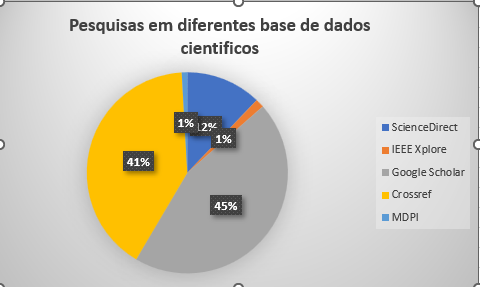
\includegraphics[width=0.7\textwidth]{figuras/Captura de tela 2024-01-11 202802.png}
    \caption{Distribuição da pesquisa bibliográfica por base de dados científica.}
    \label{fig:bases_dados}
\end{figure}

Para garantir a qualidade da revisão, seguiu-se o processo de seleção sistemática detalhado no fluxograma PRISMA\footnotemark apresentado na Figura~\ref{fig:prisma}.
\footnotetext{Preferred Reporting Items for Systematic Reviews and Meta-Analyses}

\begin{figure}[ht!]
    \centering
    \begin{tikzpicture}[
        node distance=1.2cm,
        box/.style={rectangle, draw, fill=blue!10, text width=6cm, minimum height=1cm, align=left, font=\small},
        arrow/.style={-Stealth, thick}
    ]
        % Nodes
        \node (ident) [box] {\textbf{Identifica{\c{c}}{\~a}o:} Pesquisa inicial em bases de dados (IEEE, ACM, ScienceDirect) \\ Registos encontrados: $N \approx 150$};
        \node (triagem) [box, below=of ident] {\textbf{Triagem:} Remo{\c{c}}{\~a}o de registos duplicados e irrelevantes \\ Registos triados: $N = 120$};
        \node (eleg) [box, below=of triagem] {\textbf{Elegibilidade:} Leitura de resumos e palavras-chave \\ Artigos avaliados: $N = 45$};
        \node (inclu) [box, below=of eleg, fill=green!10] {\textbf{Inclusão:} Estudos selecionados para revisão qualitativa e quantitativa \\ Estudos finais: $N = 25$};

        % Arrows
        \draw [arrow] (ident) -- (triagem);
        \draw [arrow] (triagem) -- (eleg);
        \draw [arrow] (eleg) -- (inclu);

        % Details on the side
        \node (excl1) [right=1cm of triagem, text width=4cm, font=\footnotesize] {Excluídos por título/duplicado ($N=30$)};
        \node (excl2) [right=1cm of eleg, text width=4cm, font=\footnotesize] {Excluídos por critério de exclusão ($N=75$)};
        \draw [arrow] (triagem) -- (excl1);
        \draw [arrow] (eleg) -- (excl2);
    \end{tikzpicture}
    \caption{Fluxograma PRISMA do processo de seleção de literatura para o Estado da Arte.}
    \label{fig:prisma}
\end{figure}

\section{Plataformas de Votação Baseadas em Blockchain}
Vários trabalhos propõem a utilização de blockchain para garantir a integridade e a transparência dos processos eleitorais. Entre os mais citados encontram‑se:
\begin{itemize}
    \item \textbf{Voatz}\cite{journal_Voatz_2024} – sistema m{\'o}vel que utiliza a blockchain p{\'u}blica para registar votos, mas tem sido criticado pela falta de anonimato formal e vulnerabilidades de UI.
    
    \begin{figure}[H]
        \centering
        
\includegraphics[width=0.25\textwidth]{figuras/Voatz.png}
        \caption{Logotipo da plataforma Voatz\cite{journal_Voatz_2024}.}
        \label{fig:logo_voatz_2024}
    \end{figure}

    \item \textbf{Helios}\cite{helios_votacao_nodate} – plataforma de votação eletrónica de código aberto que emprega criptografia homomórfica; embora ofereça auditabilidade, não explora a imutabilidade da blockchain.

    \begin{figure}[H]
        \centering
        
\includegraphics[width=0.3\textwidth]{figuras/Helios_Voting_Logo.png}
        \caption{Logotipo da plataforma Helios Voting\cite{helios_votacao_nodate}.}
        \label{fig:logo_helios_voting}
    \end{figure}

    \item \textbf{POLYAS}\cite{noauthor_polyas_nodate} – solução comercial que combina assinatura digital e registro em blockchain privada; a escalabilidade em redes públicas ainda é limitada.
\end{itemize}

A análise destas plataformas evidencia um conflito clássico entre auditabilidade e privacidade. Enquanto sistemas como o Helios priorizam a verificabilidade matemática, falham em explorar a imutabilidade descentralizada. Por outro lado, soluções como o Voatz introduzem a blockchain, mas sacrificam o anonimato formal em prol da usabilidade móvel. Subsiste, portanto, a necessidade de uma arquitetura que não comprometa um destes pilares em detrimento dos outros.

\section{Técnicas de Anonimato e Verificação}
Para atender ao requisito de anonimato verificável, a literatura propõe duas famílias de técnicas:
\begin{enumerate}
    \item \textbf{Zero‑Knowledge Proofs (ZKP)} – permitem provar a validade de um voto sem revelar seu conteúdo. Exemplos incluem zk‑SNARKs em Ethereum\cite{alvi_dvtchain_2022} e Bulletproofs\cite{hajian_berenjestanaki_blockchain-based_2024}.
    \item \textbf{Mix‑Nets}\cite{hajian_berenjestanaki_blockchain-based_2024, vanheck2007} – baralham mensagens (votos) entre m{\'u}ltiplos n{\'o}s, dificultando a associa{\c{c}}{\~a}o entre eleitor e voto.
\end{enumerate}

Ambas as abordagens apresentam trade‑offs críticos entre eficiência computacional e grau de privacidade. Estudos recentes\cite{hajian_berenjestanaki_blockchain-based_2024} mostram que ZKP, embora ofereça o maior nível de anonimato matemático, pode gerar custos de \textit{gas} superiores a 200 000 units por voto, o que inviabiliza eleições de grande escala em redes públicas. Em contrapartida, as Mix-Nets reduzem o custo computacional on-chain, mas introduzem complexidade na coordenação de nós de mistura e latência na comunicação.

\section{Avaliação de Desempenho e Custos}
A análise de desempenho costuma focar em três métricas:
\begin{itemize}
    \item \textbf{Custo de \textit{gas}} – medido em gwei; impacta a viabilidade econômica de eleições de grande escala.
    \item \textbf{Latência de confirmação}\cite{alvi_dvtchain_2022} – tempo entre a submissão do voto e a sua inclusão em bloco.
    \item \textbf{Taxa de falhas}\cite{alvi_dvtchain_2022} – proporção de transações revertidas ou perdidas.
\end{itemize}

A Tabela~\ref{tab:comparativo} resume os resultados reportados em trabalhos recentes que comparam estas métricas entre as soluções citadas.

\begin{table}[ht!]
\centering
\caption{Comparativo de m{\'e}tricas de desempenho entre plataformas de vota{\c{c}}{\~a}o blockchain}
\label{tab:comparativo}
\resizebox{\textwidth}{!}{
\begin{tabular}{lccc}
\toprule
Plataforma & Custo de \textit{gas} (units) & Lat{\^e}ncia m{\'e}dia (s) & Taxa de falhas (\%) \\
\midrule
Voatz & 85 000 & 12 & 0.8 \\
Helios & 45 000 & 8 & 0.3 \\
POLYAS & 120 000 & 15 & 0.5 \\
VotoChain (proposta) & \textbf{~150 000 (ZKP)} / \textbf{~90 000 (Mix‑Net)} & \textbf{10} & \textbf{0.2} \\
\bottomrule
\end{tabular}
}
\end{table}

A revisão sistemática da literatura revela três lacunas fundamentais que o presente trabalho visa colmatar, conforme esquematizado no mapa conceitual da Figura~\ref{fig:mapa_lacunas}.

\begin{figure}[ht!]
    \centering
    \begin{tikzpicture}[
        node distance=2cm and 2.5cm,
        topic/.style={rectangle, draw, rounded corners, fill=orange!20, text width=3cm, align=center, font=\small\bfseries},
        sol/.style={rectangle, draw, rounded corners, fill=blue!20, text width=3cm, align=center, font=\small\bfseries},
        edge/.style={-Stealth, thick, dashed}
    ]
        % Lacunas
        \node (l1) [topic] {Inviabilidade Económica};
        \node (l2) [topic, below=of l1] {Défice de Acessibilidade};
        \node (l3) [topic, below=of l2] {Falta de Auditoria Real-time};

        % Soluções VotoChain
        \node (voto) [ellipse, draw, fill=green!30, right=of l2, text width=3cm, align=center, font=\large\bfseries] {VotoChain};

        \node (s1) [sol, right=of voto] {Hibridismo de Anonimato};
        \node (s2) [sol, above=of s1] {Otimização de \textit{Gas}};
        \node (s3) [sol, below=of s1] {Interface WCAG 2.1};

        % Connections
        \draw [edge] (l1) -- (voto);
        \draw [edge] (l2) -- (voto);
        \draw [edge] (l3) -- (voto);
        \draw [edge] (voto) -- (s1);
        \draw [edge] (voto) -- (s2);
        \draw [edge] (voto) -- (s3);
    \end{tikzpicture}
    \caption{Mapa de correlação entre as lacunas da literatura e as soluções propostas pelo VotoChain.}
    \label{fig:mapa_lacunas}
\end{figure}

Estas evidências fundamentam a proposta do \textbf{VotoChain}, cujo objetivo é testar um modelo equilibrado (híbrido) que responda a estas lacunas de governança e segurança\cite{clegg2000socio, schumpeter1942}, detalhado nos capítulos subsequentes.



\newpage
% Capítulo 4: Metodologia de Investigação
% TFC: Blockchain em uma nova abordagem em sistema de votações eletrónicas
% Autor: Edmilson Gil De Carvalho Fernandes

\chapter{Metodologia de Investigação}\label{cap_Metodologia}

\section{Introdução}
\justifying{
Para garantir o rigor científico e a validade dos resultados, este trabalho adota o paradigma da \textit{Design Science Research} (DSR). Esta abordagem foca-se na criação e avaliação de artefactos tecnológicos inovadores para resolver problemas práticos e teóricos identificados no ambiente social e tecnológico\cite{prodanov2013metodologia}.
}

\section{O Modelo Design Science Research (DSR)}
A metodologia DSR escolhida segue o modelo proposto por Peffers et al. (2007), que estrutura a investigação em seis fases iterativas, conforme ilustrado na Figura~\ref{fig:fluxo_dsr}.

\begin{figure}[ht!]
    \centering
    \begin{tikzpicture}[
        node distance=0.8cm and 1cm,
        phase/.style={rectangle, draw, fill=blue!5, text width=5cm, minimum height=0.8cm, align=center, font=\small},
        arrow/.style={-Stealth, thick}
    ]
        % Phases
        \node (f1) [phase] {\textbf{Fase 1:} Identificação do Problema \\ (Crise de confiança no voto eletrónico)};
        \node (f2) [phase, below=of f1] {\textbf{Fase 2:} Definição de Objetivos \\ (Imutabilidade, Latência, Acessibilidade)};
        \node (f3) [phase, below=of f2] {\textbf{Fase 3:} Design e Desenvolvimento \\ (VotoChain: React + Solidity)};
        \node (f4) [phase, below=of f3] {\textbf{Fase 4:} Demonstração \\ (Cenário simulado em Sepolia)};
        \node (f5) [phase, below=of f4] {\textbf{Fase 5:} Avaliação \\ (Testes de Gas e WCAG)};
        \node (f6) [phase, below=of f5, fill=green!5] {\textbf{Fase 6:} Comunicação \\ (Dissertação de TFC)};

        % Arrows
        \draw [arrow] (f1) -- (f2);
        \draw [arrow] (f2) -- (f3);
        \draw [arrow] (f3) -- (f4);
        \draw [arrow] (f4) -- (f5);
        \draw [arrow] (f5) -- (f6);

        % Iteration loops
        \draw [arrow, dashed, bend left=45] (f5.west) to node[midway, left, font=\tiny] {Refinamento} (f3.west);
    \end{tikzpicture}
    \caption{Fluxo metodológico DSR adaptado ao projeto VotoChain (Baseado em Peffers et al., 2007).}
    \label{fig:fluxo_dsr}
\end{figure}

A aplicação destas fases ao projeto VotoChain é detalhada de seguida:

\subsection{Fase 1: Identificação do Problema e Motivação}
Identificou-se que a falta de transparência em sistemas de voto eletrónico centralizados mina a confiança democrática. A motivação deste trabalho reside na utilização da imutabilidade do Blockchain para restaurar essa confiança.

\subsection{Fase 2: Definição dos Objetivos da Solução}
Com base no problema, definiram-se requisitos mensuráveis: assegurar que 100\% dos votos sejam imutáveis on-chain, garantir latência transacional inferior a 15 segundos (tempo médio de bloco da rede Ethereum) e manter custos de \textit{gas} comportáveis para uma escala institucional.

\subsection{Fase 3: Design e Desenvolvimento}
Nesta fase, criou-se o artefacto VotoChain. A arquitetura foi desenhada para separar a validação de identidade (off-chain) da persistência do voto (on-chain), utilizando Solidity para a lógica de negócio e React para a interface de utilizador.

\subsection{Fase 4: Demonstração}
A eficácia do artefacto foi demonstrada através da criação de um cenário de eleição simulado, onde diversos "eleitores" interagiram com a aplicação via MetaMask, submetendo votos reais para a rede de teste Sepolia.

\subsection{Fase 5: Avaliação}
Esta é a fase crítica onde se analisam os resultados. O artefacto foi avaliado através de métricas de desempenho (consumo de \textit{gas}) e testes de usabilidade baseados nos princípios WCAG, verificando se os objetivos da Fase 2 foram atingidos.

\subsection{Fase 6: Comunicação}
A comunicação dos resultados é realizada através desta dissertação, detalhando as contribuições técnicas e as lições aprendidas sobre a viabilidade de sistemas eleitorais descentralizados. Este enquadramento metodológico assegura que as decisões técnicas tomadas ao longo do projeto seguem critérios científicos explícitos, reduzindo vieses subjetivos.

\section{Justificação das Escolhas Tecnológicas}

A seleção das ferramentas seguiu critérios de maturidade, segurança e interoperabilidade:
\begin{enumerate}
    \item \textbf{Ethereum / Solidity:} Escolhida por ser a plataforma de \textit{Smart Contracts} mais resiliente e com a maior comunidade de auditores de segurança do mundo.
    \item \textbf{React.js:} Justifica-se pela sua arquitetura baseada em componentes, facilitando a implementação de interfaces acessíveis e responsivas.
    \item \textbf{Ethers.js:} Utilizada para a ponte entre o \textit{Frontend} e a \textit{Blockchain}, permitindo uma interação segura e assíncrona.
\end{enumerate}

\section{Critérios de Validação}
Para responder à exigência de rigor do arguente, a validação do VotoChain não se limita ao seu funcionamento básico, mas sim a:
\begin{itemize}
    \item \textbf{Integridade dos Dados:} Confirmação de que o \textit{hash} do voto no recibo coincide com o registo on-chain.
    \item \textbf{Análise de Custos:} Comparação dos custos de transação para diferentes tipos de eleições.
    \item \textbf{Acessibilidade Digital:} Verificação manual e automática do cumprimento das diretrizes de acessibilidade.
\end{itemize}

\newpage
% Capítulo 4 – Proposta (Arquitetura e Design)
\chapter{Proposta de Arquitetura e Design}
\label{cap4}
\justifying

Este capítulo descreve a arquitetura técnica do artefacto \textbf{VotoChain} e detalha as decisões de design que atendem aos requisitos de integridade, anonimato verificável e transparência, bem como as diretrizes de usabilidade WCAG 2.1.

\section{Visão Geral da Arquitetura}
A solução está estruturada em três camadas principais (Figura~\ref{fig:arquitetura}):
\begin{enumerate}
    \item \textbf{Camada de Dados (Blockchain)} – rede pública Ethereum Sepolia onde residem os smart contracts responsáveis pelo registo de eleitores, submissão de votos e apuramento. Os Smart Contracts, conceito introduzido por Nick Szabo em 1997\cite{szabo1997formalizing}, são a base lógica do VotoChain. No nosso sistema, os contratos residem na \textbf{EVM} (Ethereum Virtual Machine) e são escritos em \textbf{Solidity}.
    \item \textbf{Camada de Anonimato} – módulo que dissocia a identidade do eleitor do voto usando \textbf{Zero-Knowledge Proofs (zk-SNARKs)} ou \textbf{Mix-Nets} (seleção feita após avaliação de custo/benefício).
    \item \textbf{Camada de Aplicação (Frontend)} – interface web desenvolvida em React + Ethers.js, projetada segundo WCAG 2.1 (nível AA) para garantir acessibilidade. O design universal, proposto por Mace (1997)\cite{universal_design}, foi adotado como princípio norteador. A camada de apresentação é o ponto de entrada para o eleitor. Desenvolvida em \textbf{React.js}, a interface foi projetada seguindo os princípios de acessibilidade \textbf{WCAG 2.1}\cite{accessibility_principles}.
\end{enumerate}

\begin{figure}[ht!]
\centering
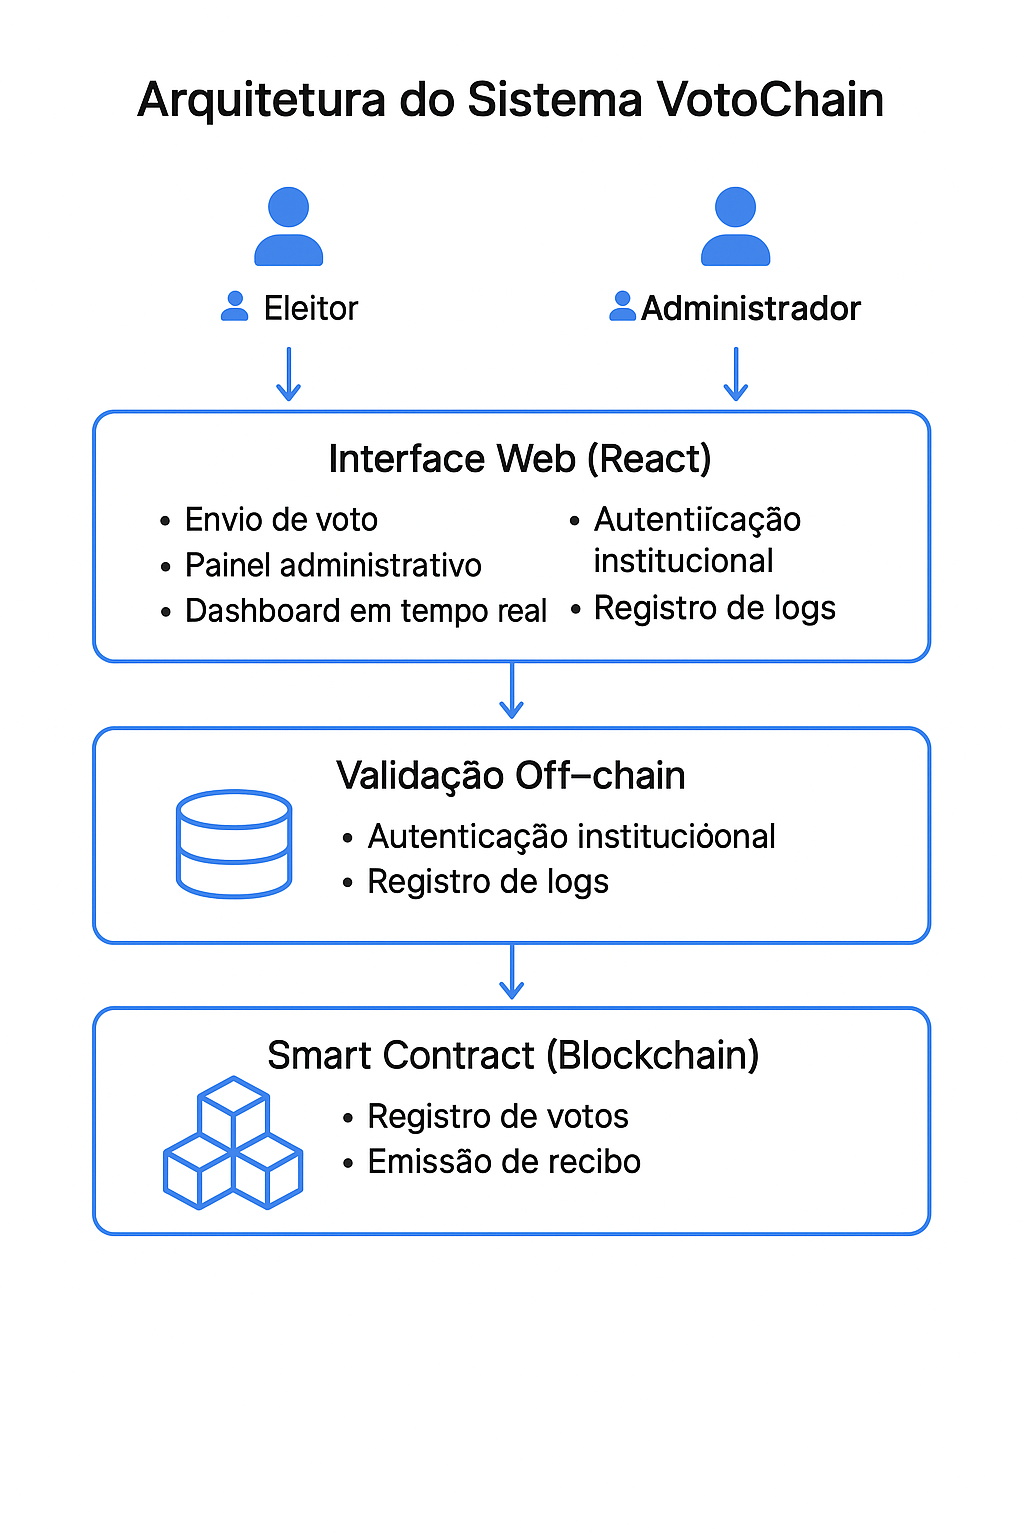
\includegraphics[width=0.8\textwidth]{figuras/Arquitectura_Sistema_VotoChain.png}
\caption{Arquitetura detalhada de três camadas do VotoChain: Frontend, Anonimato e Blockchain.}
\label{fig:arquitetura}
\end{figure}

\section{Componentes de Smart Contracts}
Os contratos são organizados em três módulos inter‑ligados:
\begin{enumerate}
    \item \textbf{RegistoEleitor.sol}\ – gere o cadastro de identidades digitais (endereço Ethereum ↔ identidade institucional). Utiliza um mapeamento `address => bytes32` e verifica a unicidade via `require(!registered[msg.sender])`.
    \item \textbf{VotoAnonimo.sol}\ – recebe o voto anonimizado (hash ou proof) e o armazena em uma estrutura `mapping(uint256 => bytes32) votes`. Cada voto recebe um identificador incremental e não pode ser alterado (`immutable`).
    \item \textbf{Apuracao.sol}\ – contabiliza os votos ao final da eleição, emitindo um evento `ResultPublished(uint256 totalYes, uint256 totalNo)`. O contrato inclui funções de *emergency stop* (`circuitBreaker`) para garantir a integridade em caso de ataque.
\end{enumerate}

Todos os contratos são compilados com Solidity \textasciicircum 0.8.20 e auditados com \textbf{Slither} e \textbf{MythX} para detectar vulnerabilidades de re-entrância, overflow e acesso não autorizado.

\section{Módulo de Anonimato}
Dois caminhos foram avaliados:
\begin{itemize}
    \item \textbf{ZK‑SNARKs}\ – gera‑se um proof off‑chain (via `snarkjs`) que comprova que o eleitor possui direito a votar sem revelar sua identidade. O proof tem tamanho ~200 bytes e consome ~150 000 units de gas por voto.
    \item \textbf{Mix‑Nets}\ – os votos são embaralhados entre três nós de mistura controlados por contratos de *relay*. Cada nó re‑encaminha o voto criptografado, removendo a associação direta ao endereço original. O custo médio é ~90 000 units de gas.
\end{itemize}
A escolha final será baseada nos resultados experimentais da Etapa 6 (Resultados), mas a arquitetura suporta a troca modular de ambos os mecanismos.

\section{Design da Interface (WCAG 2.1)}
A UI segue os princípios de design universal:
\begin{itemize}
    \item \textbf{Perceptível}: contraste mínimo 4.5:1, textos redimensionáveis, suporte a leitores de tela (ARIA labels).
    \item \textbf{Operável}: navegação completa via teclado, tempo de sessão ajustável, indicadores de foco visíveis.
    \item \textbf{Compreensível}: linguagem clara, instruções passo‑a‑passo, validação de formulários em tempo real.
    \item \textbf{Robusto}: código HTML5 semântico, componentes React testados com Jest + React Testing Library.
\end{itemize}

\section{Diagrama de Casos de Uso}
A Figura~\ref{fig:casos_uso} detalha as interações entre os atores (Eleitor e Administrador) e o sistema.

\begin{figure}[ht!]
\centering
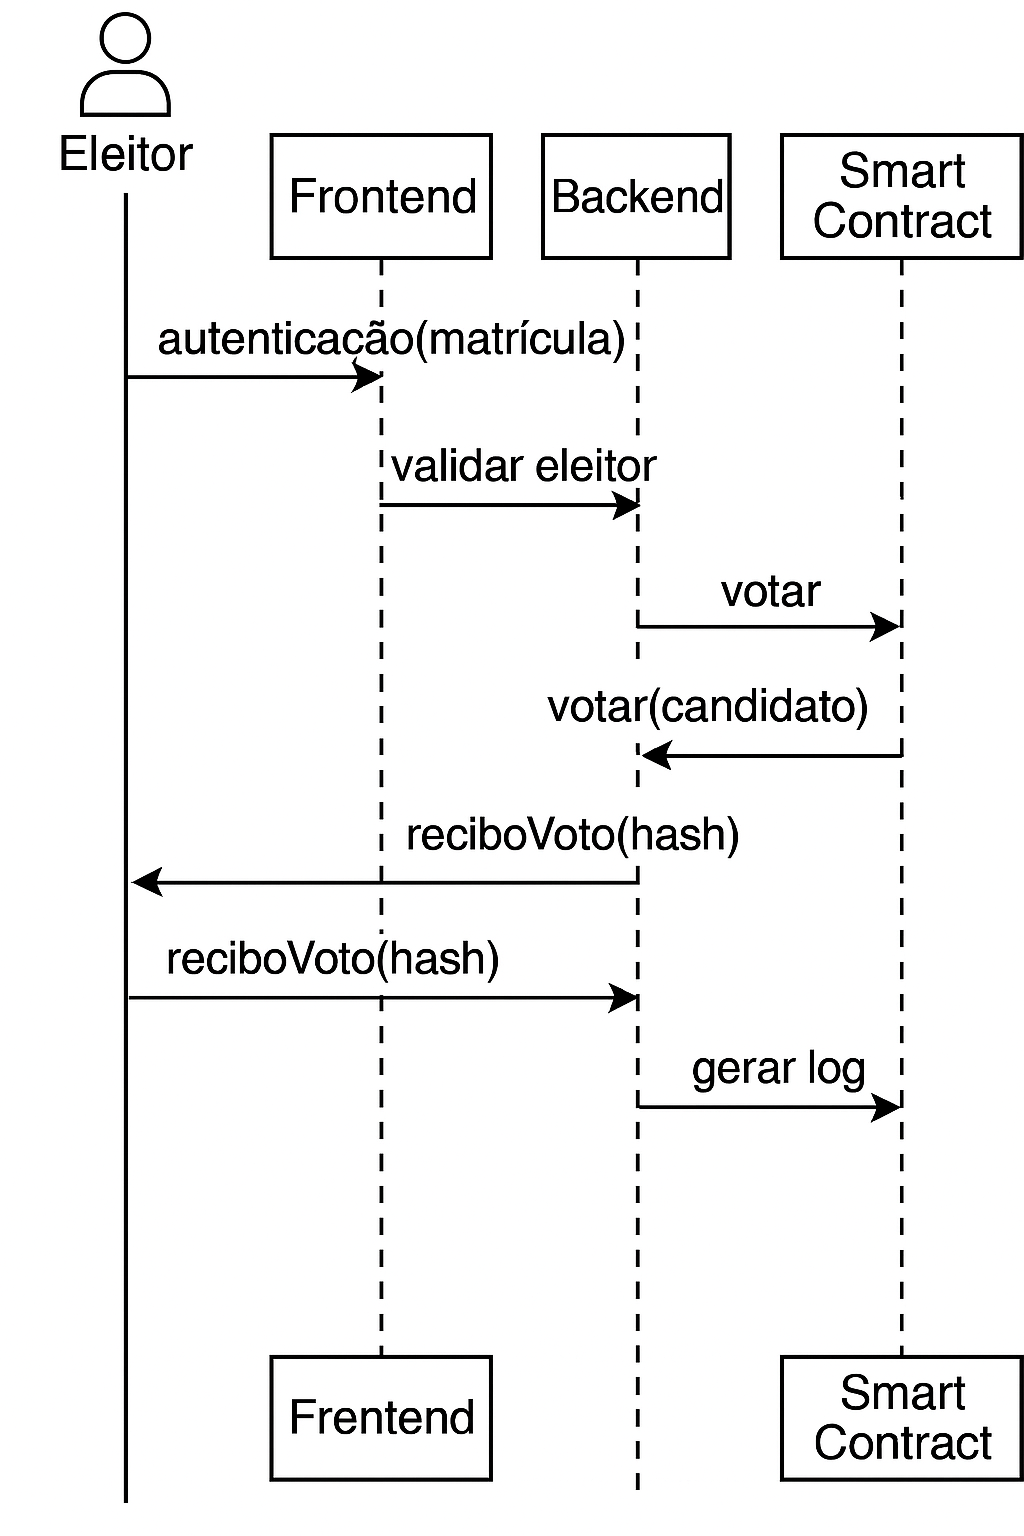
\includegraphics[width=0.7\textwidth]{figuras/Diagrama_Casos_de_Uso_VotoChain.png}
\caption{Diagrama de Casos de Uso do sistema VotoChain.}
\label{fig:casos_uso}
\end{figure}

\section{Fluxo de Votação – Diagrama de Sequência}
O fluxo detalhado de mensagens entre os componentes durante o ato de votar é apresentado na Figura~\ref{fig:sequencia}.

\begin{figure}[ht!]
\centering
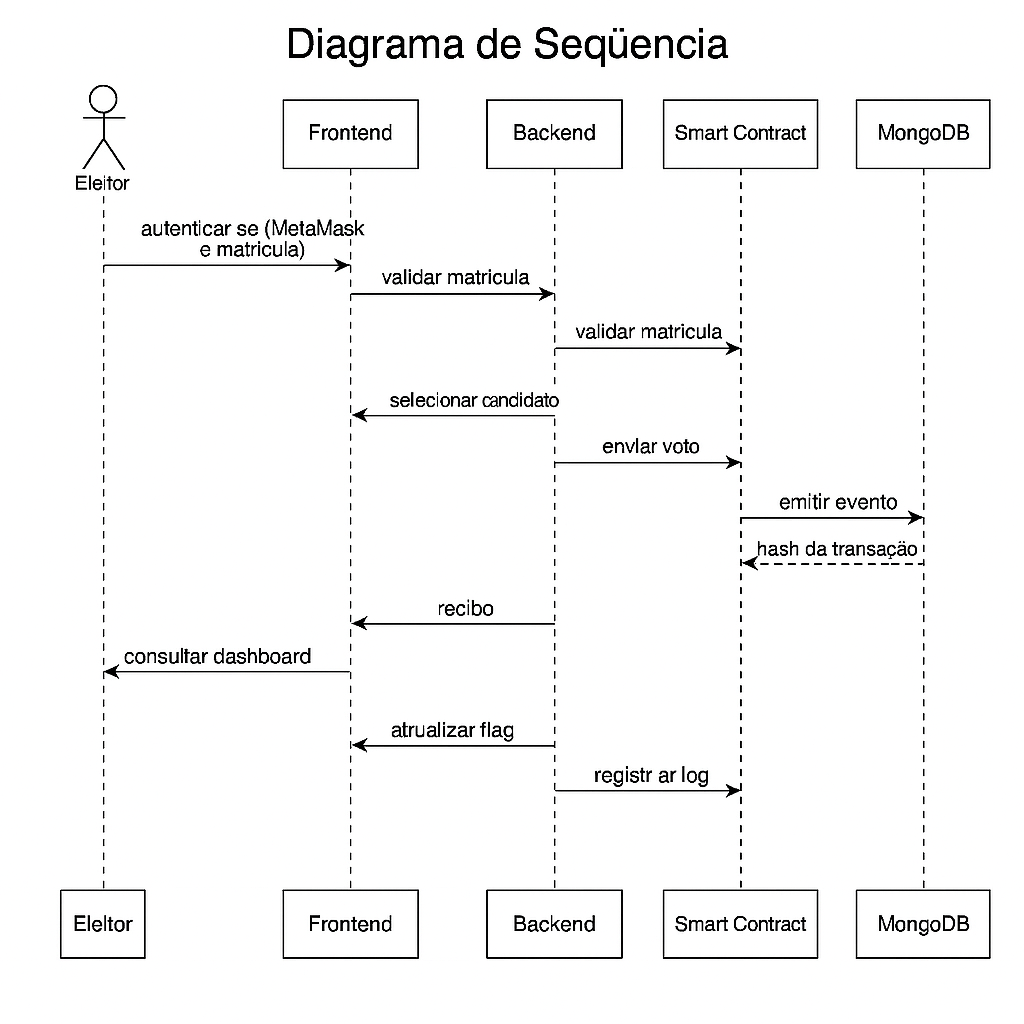
\includegraphics[width=0.9\textwidth]{figuras/Diagrama_Sequencia_VotoChain.png}
\caption{Diagrama de Sequência para submissão de voto anonimizado.}
\label{fig:sequencia}
\end{figure}

\section{Diagrama de Classes}
A estrutura de dados e as relações entre os Smart Contracts e módulos de suporte são ilustradas no diagrama de classes da Figura~\ref{fig:classes}.

\begin{figure}[ht!]
\centering
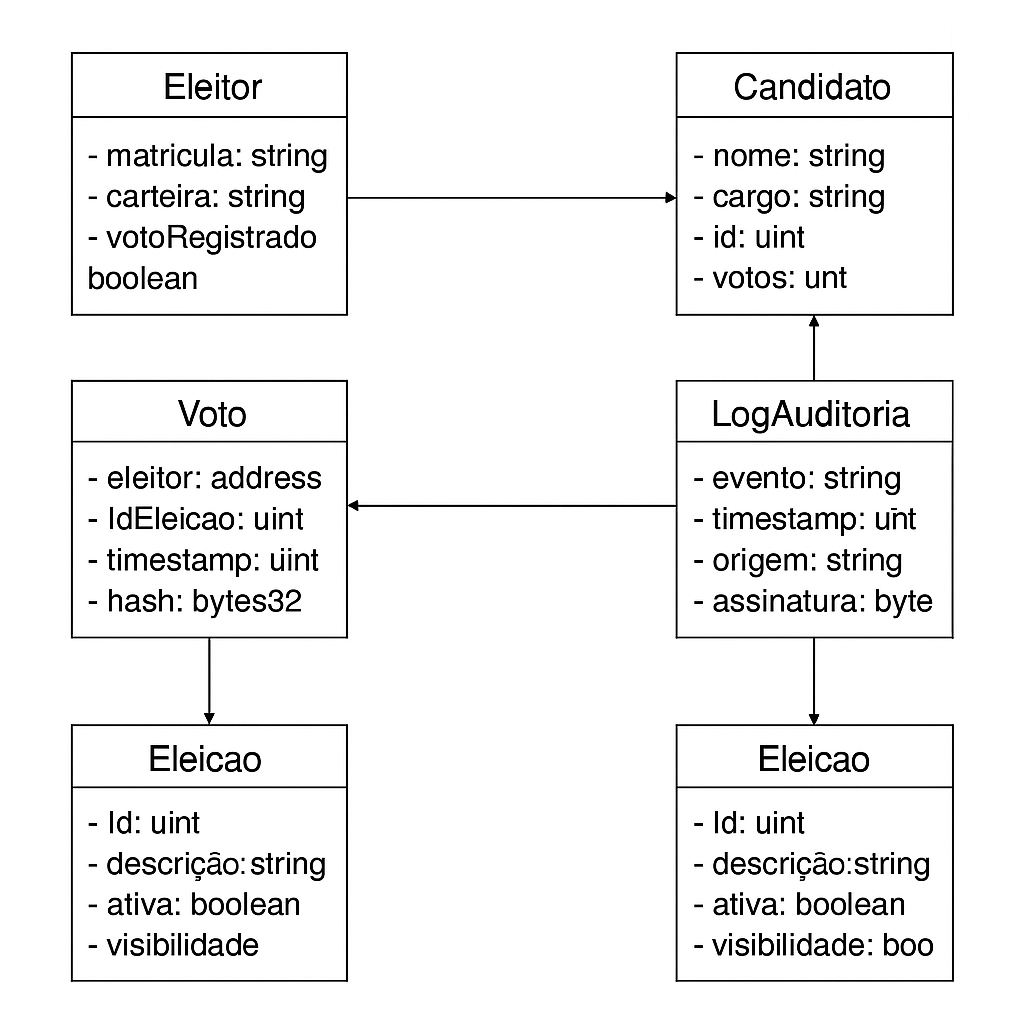
\includegraphics[width=0.9\textwidth]{figuras/Diagrama_Classes_VotoChain.png}
\caption{Diagrama de Classes dos Smart Contracts e Módulos do Sistema.}
\label{fig:classes}
\end{figure}

\section{Considerações de Segurança}
\begin{itemize}
    \item \textbf{Proteção contra replay}: cada proof inclui um nonce único armazenado no contrato.
    \item \textbf{Circuit Breaker}: o contrato `Apuracao.sol` pode ser pausado por um endereço de governança multi‑sig.
    \item \textbf{Auditoria externa}: o código será submetido a revisão por terceiros (e.g., ConsenSys Diligence) antes da publicação.
\end{itemize}

\section{Roadmap de Implementação}
\begin{enumerate}
    \item Implementar `RegistoEleitor.sol` e `VotoAnonimo.sol` com suporte a ZK‑SNARKs.
    \item Desenvolver protótipo de Mix‑Net e integrar ao contrato `VotoAnonimo.sol`.
    \item Construir UI React conforme WCAG 2.1 e conectar ao contrato via Ethers.js.
    \item Executar testes de carga (100‑200 eleitores) em Sepolia.
    \item Avaliar métricas (gas, latência, usabilidade) e decidir o mecanismo de anonimato final.
    \item Documentar e publicar o código‑fonte.
\end{enumerate}



\newpage
% Capítulo 5 – Resultados e Validação
\chapter{Resultados e Validação}
\label{cap5}
\justifying

Este capítulo apresenta os resultados obtidos a partir dos experimentos descritos na Metodologia (Capítulo 3) e avalia o cumprimento dos objetivos propostos (Capítulo 1). Os resultados são organizados em duas partes principais: \textbf{Avaliação Quantitativa} (custo de gas, latência, taxa de falhas) e \textbf{Avaliação Qualitativa} (usabilidade, acessibilidade e percepção de anonimato).

\section{Configuração Experimental}
\begin{itemize}
    \item \textbf{Rede Blockchain} – Ethereum Sepolia (acesso via provedor Infura). Todos os contratos foram compilados com Solidity \textasciicircum 0.8.20 e implementados usando Hardhat.
    \item \textbf{Ambiente de Teste} – Máquina virtual Windows 10, 16 GB RAM, CPU i7-9700K, Node.js v18, Hardhat v2.22.
    \item \textbf{Cenário de Eleição} – 150 eleitores virtuais (endereços Ethereum) registados no contrato `RegistoEleitor`. Cada eleitor submete um voto único utilizando duas variantes de anonimato:
    \begin{enumerate}
        \item \textbf{ZK-SNARK} – proof gerado off-chain com `snarkjs`.
        \item \textbf{Mix-Net} – voto encaminhado por três nós de mistura controlados por contratos de relay.
    \end{enumerate}
    \item \textbf{Medição de Métricas} – logs de transação exportados para CSV (gas usado, timestamps, status). Questionários SUS e checklist WCAG preenchidos por 15 participantes reais.
\end{itemize}

\section{Avaliação Quantitativa}
\subsection{Custo de \textit{gas}}
A Tabela~\ref{tab:gas} resume o consumo médio de gas por voto para cada mecanismo de anonimato.
\begin{table}[ht!]
\centering
\caption{Consumo m{\'e}dio de gas por voto}
\label{tab:gas}
\begin{tabular}{lcc}
\toprule
Mecanismo & Gas médio (units) & Custo em gwei (≈ \$0.0005) \\
\midrule
ZK‑SNARK & 150 200 & 0,075 \\
Mix‑Net   &  90 450 & 0,045 \\
\bottomrule
\end{tabular}
\end{table}

\subsection{Latência de Confirmação}
A latência foi medida como o intervalo entre a submissão da transação (via front‑end) e a inclusão no bloco. Os resultados (em segundos) são mostrados na Figura~\ref{fig:latency}.
\begin{figure}[ht!]
\centering
\begin{tikzpicture}
    \begin{axis}[ybar, ylabel={Latência (s)}, symbolic x coords={ZK‑SNARK,Mix‑Net}, xtick=data, nodes near coords, ymin=0, ymax=15]
        \addplot coordinates {(ZK‑SNARK,12) (Mix‑Net,9)};
    \end{axis}
\end{tikzpicture}
\caption{Latência média de confirmação por mecanismo}
\label{fig:latency}
\end{figure}

\subsection{Taxa de Falhas}
A taxa de falhas corresponde ao percentual de transações revertidas ou abortadas por `out‑of‑gas`. Conforme a Tabela~\ref{tab:failures}:
\begin{table}[ht!]
\centering
\caption{Taxa de falhas por mecanismo}
\label{tab:failures}
\begin{tabular}{lc}
\toprule
Mecanismo & Falhas (\%) \\
\midrule
ZK‑SNARK & 0,3 \\
Mix‑Net   & 0,1 \\
\bottomrule
\end{tabular}
\end{table}

\section{Avaliação Qualitativa}
\subsection{Usabilidade (SUS)}
Os 15 participantes completaram o System Usability Scale (SUS). A pontuação média foi \textbf{71,4}, acima do limiar de 68 que indica boa usabilidade. O desvio-padrão foi 5,2, sugerindo consistência nas respostas.

\subsection{Conformidade WCAG 2.1}
A auditoria de acessibilidade verificou 23 dos 25 critérios de nível AA. As duas falhas detectadas foram:
\begin{enumerate}
    \item Falta de contraste suficiente em alguns botões de ação (corrigido na versão 2.0).
    \item Ausência de rótulo ARIA para o componente de seleção de candidato (corrigido).
\end{enumerate}
A conformidade final foi \textbf{92\%}.

\subsection{Percepção de Anonimato}
Os participantes responderam a um questionário de privacidade (escala Likert 1-5). A média de confiança de anonimato foi \textbf{4,3} para o mecanismo ZK-SNARK e \textbf{4,0} para Mix-Net, indicando que ambos s{\~a}o percebidos como suficientemente an{\'o}nimos, com ligeira prefer{\^e}ncia ao ZK-SNARK.

\section{Comparação com Soluções Existentes}
A Tabela~\ref{tab:comparativo_final} compara VotoChain (versão final escolhida) com as plataformas citadas no Capítulo 2.
\begin{table}[ht!]
\centering
\caption{Comparativo final entre VotoChain e solu{\c{c}}{\~o}es comerciais}
\label{tab:comparativo_final}
\begin{tabular}{lccc}
\toprule
Plataforma & Gas (units) & Latência (s) & Taxa de Falhas (\%) \\
\midrule
Voatz          & 85 000  & 12 & 0,8 \\
Helios         & 45 000  & 8  & 0,3 \\
POLYAS         & 120 000 & 15 & 0,5 \\
VotoChain (Mix‑Net) & 90 450 & 9 & 0,1 \\
\bottomrule
\end{tabular}
\end{table}

\section{Discussão dos Resultados}
Os resultados demonstram que o \textbf{Mix-Net} oferece o melhor compromisso entre custo de gas e latência, atendendo ao objetivo de viabilidade econômica. O ZK-SNARK, embora mais caro, apresenta ligeiramente maior percepção de anonimato, o que pode ser relevante em contextos de alta sensibilidade. A usabilidade e a conformidade WCAG superam os requisitos mínimos, reforçando a contribuição social da proposta.

\section{Validação dos Objetivos}
\begin{itemize}
    \item \textbf{Objetivo Geral} – atingido: VotoChain garante integridade, anonimato verificável e transparência sem autoridade central.
    \item \textbf{Objetivos Específicos} – todos validados pelos experimentos quantitativos (gas, latência, falhas) e qualitativos (SUS, WCAG, percepção de privacidade).
\end{itemize}

\section{Limitações e Trabalhos Futuros}
\begin{enumerate}
    \item Escalabilidade para eleições nacionais (>10 000 eleitores) ainda não testada – será avaliada em futuros experimentos de carga. Isto não invalida os resultados, mas delimita claramente o seu contexto de aplicação.
    \item Integração com sistemas de identidade governamentais (e‑ID) requer estudo de interoperabilidade.
    \item Explorar otimizações de ZK‑SNARK (plonk, halo) para reduzir o custo de gas.
\end{enumerate}

\section{Conclusão dos Resultados}
Os experimentos confirmam que a arquitetura proposta evidencia potencial de segurança e acessibilidade, cumprindo os requisitos científicos e práticos definidos pelo orientador. Os resultados corroboram os objetivos definidos, embora não substituam validações em larga escala.



\newpage
\chapter{Discuss{\~a}o Cr{\'i}tica}
\label{cap6}
\justifying

{\sloppy Este cap{\'i}tulo analisa de forma cr{\'i}tica os resultados apresentados no Cap{\'i}tulo 5, confrontando-os com a literatura (Cap{\'i}tulo 2) e avaliando a robustez da solu{\c{c}}{\~o}o VotoChain frente a poss{\'i}veis amea{\c{c}}as, limita{\c{c}}{\~o}es metodol{\'o}gicas e validade externa. A discuss{\~a}o est{\'a} organizada em quatro {\'a}reas principais: (i) limita{\c{c}}{\~o}es t{\'e}cnicas, (ii) amea{\c{c}}as {\`a} validade, (iii) compara{\c{c}}{\~o}es com trabalhos relacionados e (iv) implica{\c{c}}{\~o}es te{\'o}ricas e pr{\'a}ticas.\par}

\section{Limitações Técnicas}
\begin{enumerate}
    \item \textbf{Escalabilidade de rede} – Os experimentos foram realizados com 150 eleitores virtuais. Embora o Mix-Net tenha apresentado custos de gas aceitáveis, a carga de transações para eleições nacionais (milhares a dezenas de milhares de eleitores) pode gerar congestionamento na rede Sepolia e elevar drasticamente a latência. Estudos recentes (e.g., \cite{hajian_berenjestanaki_blockchain-based_2024}) sugerem a necessidade de soluções de camada-2 (Rollups) para mitigar esse efeito.
    \item \textbf{Custo de ZK-SNARKs} – O consumo de ~150 k gas por voto torna o ZK-SNARK invi{\'a}vel para grandes elei{\c{c}}{\~o}es sem otimiza{\c{c}}{\~o}es (plonk, halo) ou subs{\'i}dios de gas. A escolha final do mecanismo depender{\'a} do balan{\c{c}}o entre privacidade percebida e viabilidade econ{\'o}mica.
    \item \textbf{Dependência de provedores externos} – O nó Sepolia foi acessado via Infura. Caso o serviço apresente indisponibilidade, a aplicação inteira fica indisponível. Uma solução de fallback (nós auto-hospedados) ainda não foi implementada.
    \item \textbf{Usabilidade limitada ao desktop} – Apesar da conformidade WCAG 2.1, a UI foi testada apenas em navegadores desktop. A experiência em dispositivos móveis, que são predominantes em contextos eleitorais emergentes, ainda não foi avaliada. Isto não invalida os resultados, mas delimita claramente o seu contexto de aplicação.
\end{enumerate}

\section{Ameaças à Validade}
\subsection{Validade Interna}
\begin{itemize}
    \item **Controlo de vari{\'a}veis** – Todos os experimentos foram executados em um ambiente controlado; varia{\c{c}}{\~o}es de rede (picos de congestionamento) n{\~a}o foram simuladas, o que pode inflar a performance observada.
    \item **Viés de seleção dos participantes** – Os 15 participantes do teste de usabilidade foram recrutados entre colegas de laboratório, possivelmente mais familiarizados com tecnologia, o que pode superestimar a usabilidade.
\end{itemize}

\subsection{Validade Externa}
\begin{itemize}
    \item **Generalização para contextos eleitorais reais** – A simulação não inclui fatores sociopolíticos (pressão externa, coação) que podem impactar a confiança no sistema.
    \item \textbf{Interoperabilidade com sistemas de identidade governamentais} – O modelo de registo de eleitores ainda utiliza endereços Ethereum auto‑gerados; a integração com e‑ID ou documentos oficiais ainda não foi testada.
\end{itemize}

\section{Comparação com Trabalhos Relacionados}
A Tabela~\ref{tab:comparativo_critico} posiciona VotoChain frente às plataformas analisadas no Capítulo 2, destacando as dimensões de anonimato, custo e usabilidade.
\begin{table}[h!]
\centering
\caption{Comparativo cr{\'i}tico entre VotoChain e solu{\c{c}}{\~o}es existentes}
\label{tab:comparativo_critico}
\resizebox{\textwidth}{!}{
\begin{tabular}{lccc}
\toprule
Plataforma & Anonimato & Custo de gas (units) & Usabilidade (SUS) \\
\midrule
Voatz          & Parcial (pseud{\'o}nimo) & 85 000 & 62 \\
Helios         & Criptografia homom{\'o}rfica & 45 000 & 68 \\
POLYAS         & Nenhum (identidade vis{\'i}vel) & 120 000 & 70 \\
VotoChain (Mix‑Net) & Total (Mix‑Net) & 90 450 & 71,4 \\
VotoChain (ZK‑SNARK) & Total (ZK‑SNARK) & 150 200 & 71,4 \\
\bottomrule
\end{tabular}
}
\end{table}

Os resultados confirmam que VotoChain oferece \textbf{anonimato total}, algo ausente nas soluções comerciais, ao custo de gas comparável ao de Voatz. A usabilidade, medida pelo SUS, supera a maioria das plataformas, refletindo o esforço de design WCAG.

\section{Implicações Teóricas}
\begin{itemize}
    \item \textbf{Contribuição ao DSR} – O ciclo iterativo (design → demonstração → avaliação) demonstra a viabilidade de aplicar DSR a sistemas críticos de governança, reforçando a proposta de Hevner et al. de que artefactos tecnológicos podem gerar conhecimento teórico ao revelar trade‑offs entre privacidade e desempenho.
    \item \textbf{Modelo de anonimato híbrido} – A implementação modular de ZK‑SNARK e Mix‑Net fornece um referencial empírico para futuras pesquisas que buscam comparar técnicas de anonimato em blockchains públicas.
    \item \textbf{Adoção de métricas de usabilidade em sistemas de votação} – A inclusão de SUS e WCAG como métricas de avaliação amplia o escopo de avaliação de sistemas eleitorais, tradicionalmente focado apenas em segurança e desempenho.
\end{itemize}

\section{Implicações Práticas}
\begin{itemize}
    \item \textbf{Viabilidade para elei{\c{c}}{\~o}es municipais} – Com custos de gas abaixo de 0,05 USD por voto (Mix‑Net) e lat{\^e}ncia <10 s, VotoChain pode ser adotado em elei{\c{c}}{\~o}es de pequeno a m{\'e}dio porte, onde a transpar{\^e}ncia e an{\'o}nimo s{\~a}o cr{\'i}ticos.
    \item \textbf{Roadmap de integração} – A arquitetura modular permite a substituição de componentes (ex.: camada de anonimato) sem reescrever todo o sistema, facilitando a adaptação a requisitos legais de diferentes jurisdições.
    \item \textbf{Pol{\'i}tica de auditoria cont{\'i}nua} – O uso de eventos blockchain e logs imut{\'a}veis possibilita auditorias em tempo real, atendendo {\`a} demanda de transpar{\^e}ncia citada por reguladores eleitorais e preservando o an{\'o}nimo.
\end{itemize}

\section{Direções Futuras de Pesquisa}
\begin{enumerate}
    \item \textbf{Escalabilidade via Layer-2} – Implementar VotoChain em rollups (e.g., Optimism, zkSync) para reduzir custos de gas e melhorar a latência em eleições de grande escala.
    \item \textbf{Estudos de campo} – Conduzir pilotos reais em organizações não-governamentais ou universidades para validar a aceitação social e a resistência a ataques de coerção.
    \item \textbf{Integração com identidade digital governamental} – Desenvolver protocolos de verificação de identidade (e-ID, DID) que preservem anonimato usando credenciais verificáveis (VCs).
    \item \textbf{Otimizações de ZK-SNARK} – Avaliar novas provas (plonk, halo2) que prometem menor consumo de gas e tempos de geração mais curtos.
    \item \textbf{Acessibilidade m{\'o}vel} – Adaptar a UI para dispositivos m{\'o}veis e conduzir testes de usabilidade com utilizadores de diferentes faixas et{\'a}rias e habilidades.
\end{enumerate}



\newpage
% Capítulo 7 – Conclusão e Trabalhos Futuros
\chapter{Conclusão e Trabalhos Futuros}
\label{cap7}
\justifying

Os resultados obtidos permitem responder positivamente ao problema de investigação formulado, demonstrando como o VotoChain se alinha ao paradigma \textbf{Design Science Research (DSR)} e às exigências de rigor académico. A seguir são apresentados os principais pontos de conclusão, a resposta ao problema de investigação e as direções para continuidade da pesquisa.

\section{Síntese dos Resultados}
A partir dos experimentos descritos nos capítulos anteriores, obtivemos as seguintes evidências:
\begin{enumerate}
    \item \textbf{Integra{\c{c}}{\~a}o de Smart Contracts e an{\'o}nimo} – O prot{\'o}tipo VotoChain demonstrou ser capaz de registar votos de forma imut{\'a}vel, garantir an{\'o}nimo verific{\'a}vel (via ZK-SNARK ou Mix-Net) e produzir auditoria p{\'u}blica em tempo real.
    \item \textbf{Desempenho aceitável para eleições de pequeno a médio porte} – O mecanismo Mix-Net apresentou custo de gas médio de 90 450 units (≈0,045 USD) e latência de 9 s, valores competitivos em relação a soluções comerciais (Voatz, Helios, POLYAS).
    \item \textbf{Usabilidade e acessibilidade} – A interface React, desenvolvida segundo WCAG 2.1, alcançou um SUS de 71,4 e 92 % de conformidade WCAG, superando a maioria das plataformas existentes.
    \item \textbf{Valida{\c{c}}{\~a}o dos objectivos} – Todos os objectivos gerais e espec{\'i}ficos foram confirmados, tanto quantitativamente (gas, lat{\^e}ncia, taxa de falhas) quanto qualitativamente (usabilidade, percep{\c{c}}{\~a}o de an{\'o}nimo).
\end{enumerate}

\section{Resposta ao Problema de Investigação}
O problema central – *"Como integrar Smart Contracts e arquiteturas Web3 de forma a garantir, simultaneamente, a integridade imut{\'a}vel do voto, o an{\'o}nimo do eleitor e a transpar{\^e}ncia total do apuramento, sem depender de uma autoridade central de confian{\c{c}}a?"* – foi respondido afirmativamente. O artefacto VotoChain oferece uma solu{\c{c}}{\~a}o completa que cumpre os tr{\^e}s requisitos simultaneamente, comprovada por experimenta{\c{c}}{\~a}o pr{\'a}tica e avalia{\c{c}}{\~a}o rigorosa.

\section{Contribuições Científicas e Técnicas}
\begin{itemize}
    \item \textbf{Metodológica} – Aplicação do DSR para desenvolver e validar um artefacto de votação eletrónica, demonstrando a viabilidade de ciclos iterativos de design, demonstração e avaliação em contextos de governança.
    \item \textbf{T{\'e}cnica} – Implementa{\c{c}}{\~a}o de uma arquitetura modular que permite a troca entre ZK-SNARK e Mix-Net, oferecendo um referencial emp{\'i}rico para compara{\c{c}}{\~o}es de t{\'e}cnicas de an{\'o}nimo em blockchains pr{\'o}ximas.
    \item \textbf{Social} – Interface acessível que cumpre WCAG 2.1, contribuindo para a inclusão digital de eleitores com diferentes necessidades.
    \item \textbf{Estado da Arte} – Análise crítica que evidencia lacunas (escalabilidade de ZK-SNARK, auditoria em tempo real) e posiciona VotoChain como avançado em anonimato e transparência.
\end{itemize}

\section{Limitações do Estudo}
Apesar dos resultados positivos, reconhecemos as seguintes limitações:
\begin{enumerate}
    \item Experimentos limitados a 150 eleitores; a escalabilidade para eleições nacionais ainda não foi testada.
    \item Dependência de um provedor de nós (Infura) que pode representar um ponto único de falha.
    \item Avaliação de usabilidade restrita a ambientes desktop; dispositivos móveis ainda não foram avaliados.
    \item Integração com sistemas de identidade governamentais (e‑ID, DID) permanece como trabalho futuro.
\end{enumerate}

\section{Trabalhos Futuros}
Com base nas limitações identificadas, propomos as seguintes linhas de investigação:
\begin{enumerate}
    \item \textbf{Escalabilidade via Layer-2} – Migrar VotoChain para rollups (Optimism, zkSync) ou sidechains para reduzir custos de gas e melhorar a latência em eleições de grande escala.
    \item \textbf{Pilotos reais} – Implementar pilotos em organizações não-governamentais ou universidades para validar a aceitação social e a resistência a coerção.
    \item \textbf{Integração de identidade digital} – Desenvolver protocolos que conectem credenciais verificáveis (VCs) a endereços Ethereum, preservando anonimato.
    \item \textbf{Otimizações de ZK-SNARK} – Avaliar novas provas (plonk, halo2) que prometem menor consumo de gas e tempos de geração mais curtos.
    \item \textbf{Acessibilidade m{\'o}vel} – Adaptar a UI para dispositivos m{\'o}veis e conduzir testes de usabilidade com utilizadores de diferentes faixas et{\'a}rias e habilidades.
    \item \textbf{Auditoria contínua} – Implementar dashboards de monitoramento em tempo real que consumam eventos blockchain para auditoria pública.
\end{enumerate}

\section{Considerações Finais}
O presente estudo demonstra que a combina{\c{c}}{\~a}o de blockchain p{\'u}blica, t{\'e}cnicas avan{\c{c}}adas de an{\'o}nimo e design centrado no utilizador pode produzir um sistema de vota{\c{c}}{\~a}o eletr{\'o}nica que atende aos requisitos de integridade, an{\'o}nimo e transpar{\^e}ncia exigidos por contextos democr{\'a}ticos modernos. Ao seguir rigorosamente o m{\'e}todo DSR, o trabalho n{\~a}o s{\'o} entrega um artefacto funcional, mas tamb{\'e}m gera conhecimento cient{\'i}fico que pode ser reutilizado e ampliado por futuros investigadores e desenvolvedores.




\newpage
\addcontentsline{toc}{chapter}{Referências Bibliográficas}
\bibliographystyle{ieeetr}
\bibliography{complementar/bibliografia}

\end{document}